% -*- LaTeX -*-
% -*- coding: utf-8 -*-
%
% michael a.g. aïvázis
% orthologue
% (c) 1998-2018 all rights reserved
%

%-----------------------------------

\section{components}
\subsection{basics}

%-----------------------------------
\begin{frame}
%
  \frametitle{Components and protocols}
%
  \begin{itemize}
%
    \item a design pattern that enables the assembly of applications out of interchangeable
      parts, under the control of the {\em end user}
      \begin{itemize}
      \item {\em protocols} are abstract specifications of application requirements
      \item {\em components} are concrete implementations that satisfy requirements
      \end{itemize}
%
    \item inversion of control:
      \begin{itemize}
      \item the binding of implementations to specifications happens at runtime, under the
        control of the end user
      \end{itemize}
%
    \item the user
      \begin{itemize}
      \item controls the application state through configuration files, the user interface, the
        command line
      \item specifies components using simple URIs
      \end{itemize}
%
    \item the goal is to isolate contributors from each other as much as possible, and provide
      a coherent and usable strategy for composing non-trivial applications
%
  \end{itemize}
%
\end{frame}

% --------------------------------------
% traits
\begin{frame}[fragile]
%
  \frametitle{Small steps: properties}
%
  \begin{itemize}
  \item let's step back and contemplate a simpler problem
%
  \begin{ipython}{}
class Disk:

    # public state
    radius = 1     # default value
    center = (0,0) # default value

    # interface
    def interior(self, points):
        ...
  \end{ipython}
%
\item what do we have to do to tie instances of \class{Disk} with information in some
  configuration file?
%
  \begin{icfg}{}
    [ disk1 ]
    center = (-1,1)   ; leave {radius} alone

    [ disk2 ]
    radius = .5
    center = (1,1)
  \end{icfg}
%
  or, equivalently, from the command line
%
  \begin{ish}{}
gauss.py --disk1.center=(1,1) --disk2.radius=.5 --disk2.center=(-1,1)
  \end{ish}
%
  \end{itemize}
%
\end{frame}

% --------------------------------------
% components:
\begin{frame}
%
  \frametitle{Components}
%
  \begin{itemize}
%
  \item informally, \emph{classes} are software specifications that establish a relationship
    between \emph{state} and \emph{behavior}
    \begin{itemize}
    \item we have syntax that allows us to specify these very close to each other
    \end{itemize}
%
  \item \emph{instances} are containers of state; there are special rules
    \begin{itemize}
    \item that grant access to this state
    \item allow you to call functions that get easy access to this state
    \end{itemize}
%
  \item \emph{components} are classes that specifically grant access to some of their state to
    the end user
    \begin{itemize}
    \item the public data are the \emph{properties} of the component
    \end{itemize}
%
  \item rule 1: components have properties
%
  \end{itemize}
%
\end{frame}

% --------------------------------------
% disk as components
\begin{frame}[fragile]
%
  \frametitle{A trivial component}
%
  \begin{itemize}
%
  \item \pyre\ provides support for writing components
%
    \begin{ipython}{}
import pyre

class Disk(pyre.component):

    # public state
    radius = pyre.properties.float(default=1)
    radius.doc = 'the radius of the disk'

    center = pyre.properties.array()
    center.default = (0,0)
    center.doc = 'the location of the center of the circle'

    # interface
    ...
    \end{ipython}
%
  \item why bother specifying the type of component properties?
    \begin{itemize}
    \item command line, configuration files, dialog boxes, web pages: they all gather
      information from the user as strings
    \item we need \emph{meta-data} so we can convert from strings to the intended object
    \end{itemize}
%
  \end{itemize}
%
\end{frame}

% --------------------------------------
% the names of things
\begin{frame}[fragile]
%
  \frametitle{The names of things}
%
  \begin{itemize}
  \item in order to connect components to configurations, we need explicit associations
    \begin{itemize}
    \item component instances have unique names
    \item component classes have unique family names
    \item namespace management: components belong to packages
    \end{itemize}
%
    \begin{ipython}{}
import pyre

class Disk(pyre.component, family="gauss.shapes.disk"):

    # public state
    radius = pyre.properties.float()
    radius.default = 1
    radius.doc = 'the radius of the disk'

    center = pyre.properties.array()
    center.default = (0,0)
    center.doc = 'the location of the center of the circle'
    ...
    \end{ipython}
%
  \item and here are a couple of component instances
%
    \begin{ipython}{}
left = Disk(name='disk1')
right = Disk(name='disk2')
    \end{ipython}
%
    \end{itemize}
%
\end{frame}

% --------------------------------------
% configuration
\begin{frame}[fragile]
%
  \frametitle{Configuration}
%
  \begin{itemize}
  \item rule 2: components have names
  \item the package name is deduced from the component family name
    \begin{itemize}
    \item it is the part up to the first delimiter
    \end{itemize}
  \item \pyre\ automatically loads configuration files whose name matches the name of a package
  \item there's even a way to override the default values that the developer hardwired into
    the class declaration
%
    \begin{icfg}{}
    [ gauss.shapes.disk ]         ; use the family name
    radius = 2                    ; to override the defaults
    center = (-1,-1)              ; for all instances of disk

    [ disk1 ]                     ; the name of an instance
    center = (-1,1)               ; leave {radius} alone

    [ disk2 ]                     ; the name of another instance
    radius = .5
    center = (1,1)
    \end{icfg}
%
  \end{itemize}
%
\end{frame}

% --------------------------------------
% recap
\begin{frame}
%
  \frametitle{Recap: what we know so far}
%
  \begin{itemize}
%
  \item \pyre\ components are evolved python objects
    \begin{itemize}
    \item the factories have family names, the instances have names
    \item these names are unique strings in hierarchical namespaces delimited by periods
    \item collections of components form packages \emph{implicitly}, based on the topmost level
      in their namespace
    \end{itemize}
%
  \item components have properties that are under the control of the \emph{user}
    \begin{itemize}
    \item they look and behave like regular attributes
    \item they are \emph{typed} to enable conversions from strings
    \item they have default values and other metadata
    \end{itemize}
%
  \item configuration is partly about assigning values to component properties
    \begin{itemize}
    \item a requirement for supporting user interfaces
    \item intuitive syntax for the command line
    \item simple configuration files inspired by the Microsoft Windows \identifier{.ini} format
    \end{itemize}
%
  \item configuration is automatically handled by the framework and requires no explicit
    involvement on the part of the component author
%
  \end{itemize}
%
\end{frame}

% --------------------------------------
% configuration files
\begin{frame}[fragile]
%
  \frametitle{Configuration files}
%
  \vskip -2ex
  \begin{itemize}
%
  \item currently, there are two file formats for configuration information
    \begin{itemize}
    \item \srcfile{.cfg}: the format in the examples
    \item \srcfile{.pml}: an \srcfile{XML} based format that is a bit more powerful but not as
      user friendly
    \end{itemize}
%
  \item \pyre\ looks for configuration files in the following places
    \begin{itemize}
    \item explicitly provided on the command line
      \begin{ish}{}
 gauss.py --config=sample.cfg
      \end{ish}
    \item the current directory
    \item the \srcfile{.pyre} subdirectory of the current user's home directory
    \item a special subdirectory wherever \pyre\ is installed
    \end{itemize}
    in order of priority
%
  \item settings on the command line have the highest priority, and override each other from
    left to right
%
  \item when a property is assigned a value multiple times, the highest priority setting wins
    \begin{itemize}
    \item the framework keeps track of all changes in the value of properties and the source of
      the assignment, so if a property doesn't end up with the value you expected, you can get
      its complete history
    \end{itemize}
%
  \end{itemize}
%
\end{frame}

% --------------------------------------
% properties
\begin{frame}
%
  \frametitle{Properties}
%
  \vskip -2ex
  \begin{itemize}
%
  \item properties make sense for both classes and instances
    \begin{itemize}
    \item the class holds the default value that gets used in case the component instance does
      not have explicit configuration
    \item each instance gets its own private value when it gets configured
    \item identical to regular python attributes
    \end{itemize}
%
  \item there is support for
    \begin{itemize}
    \item simple types: \function{bool}, \function{int}, \function{float}, \function{str}
    \item containers: \function{tuple}, \function{array}
    \item higher level: \function{date}, \function{time}, \function{inputfile},
      \function{outputfile}, \function{inet}
    \item units: \function{dimensional}
    \item easy enough to implement your own; the requirements are very simple
    \end{itemize}
%
  \item metadata:
    \begin{itemize}
    \item \identifier{doc}: a simple and short documentation string
    \item \identifier{default}: the default value, in case the user doesn't supply one
    \item \identifier{converters}: a chain of preprocessors of the string representation
    \item \identifier{normalizers}: a chain of post-processors of the converted value
    \item \identifier{validators}: a tuple of predicates that get called to ensure the property
      value satisfies the specified constraints
    \item you can add your own; the framework passes them through to your component
    \end{itemize}
%
  \end{itemize}
%
\end{frame}

% --------------------------------------
% units
\begin{frame}[fragile]
%
  \frametitle{Units}
%
  \vskip -2ex
  \begin{itemize}
%
  \item \function{dimensional} properties have units
%
  \item the low level support is in \package{pyre.units}
    \begin{itemize}
    \item full support for all SI base and derived units
    \item all common abbreviations and names from alternative systems of units
    \item correct arithmetic; proper handling of functions from \package{math}
    \end{itemize}
%
    \begin{ipython}{}
from math import cos
from pyre.units.SI import meter, second, radian

A = 2.5 * meter
t = 1.5 * second
ω = 4.2 * radian/second

x = A * cos(ω * t)
    \end{ipython}
%
    if the units in the argument to \function{cos} do not cancel, leaving a pure
    \keyword{float} behind, an exception is raised; \identifier{x} has dimensions of meters
%
  \end{itemize}
%
\end{frame}

% --------------------------------------
% facilities
\begin{frame}[fragile]
%
  \frametitle{Connecting components}
%
  \vskip -2ex
  \begin{itemize}
%
  \item the real power is in wiring components to other components
%
    \begin{ipython}{}
import pyre

class MonteCarlo(pyre.component, family="gauss.integrators.montecarlo"):
    """
    A Monte Carlo integrator
    """

    # public state
    samples = pyre.properties.int(default=10**5)
    region = ????
    ...
    \end{ipython}
%
  \item \component{MonteCarlo} should be able to specify what constitutes an acceptable region
  \item \component{Disk} should be able to advertise itself as being an acceptable
    region
  \item the user should have natural means for specifying that she wants to wire an instance of
    \component{Disk} as the region of integration
  \item and be able to configure that particular instance of \component{Disk} in a natural
    manner
  \item the framework should check the consistency of this assignment
  \end{itemize}
%
\end{frame}

% --------------------------------------
% protocols
\begin{frame}
%
  \frametitle{Protocols}
%
  \vskip -2ex
  \begin{itemize}
%
  \item the component version of an abstract base class is the \emph{protocol}
%
    \python{firstnumber=9,linerange={9-39},basicstyle=\tt\tiny}%
           {../../examples/gauss.pyre/gauss/shapes/Shape.py}
%
  \end{itemize}
%
\end{frame}

% --------------------------------------
% disk revisited
\begin{frame}[fragile]
%
  \frametitle{Declaring compatibility with a protocol}
%
  \vskip -2ex
  \begin{itemize}
%
  \item \component{Disk} can inform the framework that it intends to implement
    \protocol{Shape}
%
    \begin{ipython}{}
import pyre
from .Shape import Shape

class Disk(pyre.component, family="gauss.shapes.disk", implements=Shape):
    """
    A representation of a circular disk
    """

    ...
    \end{ipython}
%
  \item an exception is raised if \component{Disk} does not conform fully to \protocol{Shape}
%
    \begin{itemize}
    \item missing methods or missing attributes
    \end{itemize}
%
  \item also, proper namespace design simplifies many things for the user
%
    \begin{itemize}
    \item \protocol{Shape} declared its family as \identifier{gauss.shapes}
    \item \component{Disk} declared its family as \identifier{gauss.shapes.disk}
    \end{itemize}
%
  \item we'll see how later when it's time to put all this together
%
  \end{itemize}
%
\end{frame}

% --------------------------------------
% facilities
\begin{frame}[fragile]
%
  \frametitle{Specifying assignment requirements}
%
  \vskip -2ex
  \begin{itemize}
%
  \item \component{MonteCarlo} can now specify it expects a \protocol{Shape} compatible object
    to be assigned as its region of integration
%
    \begin{ipython}{}
import pyre
from .Shape import Shape

class MonteCarlo(pyre.component, family="gauss.integrators.montecarlo"):
    """
    A Monte Carlo integrator
    """

    # public state
    samples = pyre.properties.int(default=10**5)
    region = Shape()
    ...
    \end{ipython}
%
  \item the default value is whatever \protocol{Shape} returns from its
    \function{pyre\_default} class method
%
  \end{itemize}
%
\end{frame}

% --------------------------------------
% component specification
\begin{frame}[fragile]
%
  \frametitle{Component specification}
%
  \vskip -2ex
  \begin{itemize}
%
  \item and now for the real trick: converting some string provided by the user into a live
    instance of \component{Disk}, configuring it, and attaching it to some
    \component{MonteCarlo} instance
%
  \item the syntax is motivated by \identifier{URI}, the universal resource identifiers of the
    web; the general form is
    \begin{icfg}{}
      <scheme>://<authority>/<path>#<identifier>
    \end{icfg}
    where most of the segments are optional
%
  \item if your component is accessible from your python path, you could specify
    \begin{icfg}{}
      import:gauss.shapes.disk
    \end{icfg}
%
  \item if your component instance is somewhere on your disk, you would specify
    \begin{icfg}{}
      file:/tmp/shapes.py/disk
    \end{icfg}
%
  \item in either case, \function{disk} is expected to be a name that resolves into a component
    class, a component instance or be a callable that returns one of these
%
  \end{itemize}
%
\end{frame}

% --------------------------------------
% the user does the wiring
\begin{frame}[fragile]
%
  \frametitle{The user does the wiring}
%
  \vskip -2ex
  \begin{itemize}
%
  \item with our definition of \component{MonteCarlo}, an appropriately structured package
    \package{gauss} on the python path, and the following configuration file
%
    \begin{icfg}{}
 [ gauss.shapes.disk ] ; change the default values for all disks
 radius = 1
 center = (0,0)

 [ mc ] ; configure our Monte Carlo integrator instance
 region = import:gauss.shapes.disk
 ...
    \end{icfg}{}
%
  \item the following python code in some script \srcfile{sample.py}
%
    \begin{ipython}{}
   ...
   mc = MonteCarlo(name="mc")
   ...
    \end{ipython}
%
    builds a \component{MonteCarlo} instance and configures it so that its region of
    integration is a \component{Disk} instance; similarly, from the command line
%
    \begin{ish}{}
    sample.py --mc.region=import:gauss.shapes.disk
    \end{ish}
%
    or, thanks to the consistency in our namespace layout, simply
%
    \begin{ish}{}
    sample.py --mc.region=disk
    \end{ish}
%
\end{itemize}
%
\end{frame}

%-----------------------------------

\subsection{gauss}

%-----------------------------------
\begin{frame}
%
  \frametitle{A non-trivial example}
%
  \vskip -2ex
  \begin{itemize}
  \item {\tt gauss}: an extensible numeric integration package
    \begin{itemize}
      \item specify protocols and components
      \item identify the configurable state
      \item implement component behavior in terms of the specified protocols
    \end{itemize}
  \end{itemize}
%
  \begin{figure}
    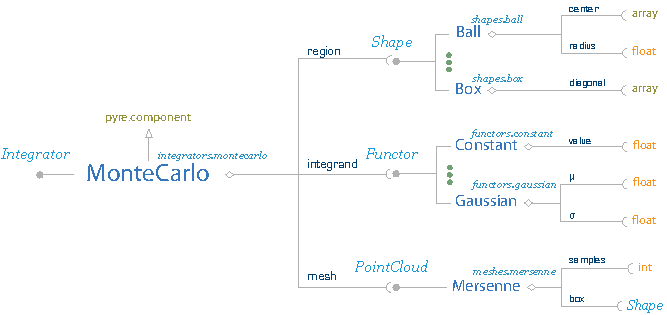
\includegraphics[scale=1.0]{figures/montecarlo.pdf}
  \end{figure}
%
\end{frame}

%-----------------------------------
\begin{frame}
%
  \frametitle{Implementation strategy}
%
  \vskip -2ex
  \begin{itemize}
%
  \item key abstractions:
    \begin{description}
    \item[functor:] encapsulation of a function in a class; our integrands will be functors
    \item[shape:] a spatial domain; we will use these to specify the region of integration
    \item[mesh:] a discretization of the domain of integration; meshes provide the locations at
      which we sample integrands
    \item[integrator:] the implementation of a particular integration algorithm
    \end{description}
%
  \item each one of these will turn into a {\em protocol}
    \begin{itemize}
    \item that spells out all the obligations imposed on concrete realizations
    \end{itemize}
%
  \item the various package {\em components}
    \begin{itemize}
    \item will provide concrete implementations of all the obligations
    \item and specify their public state: what can be delegated to the end user
    \end{itemize}
%
  \end{itemize}
%
\end{frame}

% --------------------------------------
% namespace design
\begin{frame}
%
  \frametitle{Namespace design}
%
  \vskip -2ex
  \begin{itemize}
%
  \item we are now in a position to assemble the package \package{gauss}; let's start by laying
    out the package namespace
%
  \begin{figure}
    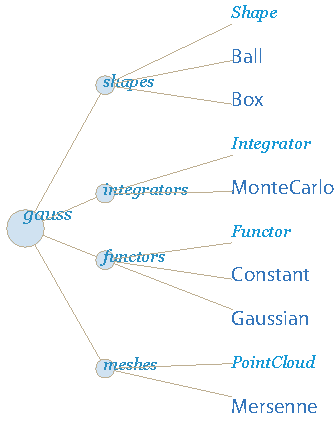
\includegraphics[scale=0.5]{figures/layout-namespace.pdf}
  \end{figure}
%
  \item and try to use this layout for both the logical and physical structure
    \begin{itemize}
    \item the top level is our package name
    \item the internal nodes become the names of interfaces and subdirectories
    \item the leaves are the component family names and the names by which the component
      factories are accessible
    \end{itemize}
%
  \end{itemize}
%
\end{frame}

% --------------------------------------
% shape as a package
\begin{frame}[fragile]
%
  \frametitle{The \package{shapes} package}
%
  \vskip -2ex
  \begin{itemize}
%
  \item in order to make the directory \srcfile{gauss/shapes} a python package, we need to
    create the special file \srcfile{gauss/shapes/\_\_init\_\_.py}
%
    \python{firstnumber=9,linerange={9-18}}{../../examples/gauss.pyre/gauss/shapes/__init__.py}
%
  \item the \keyword{import} statements
    \begin{itemize}
    \item use \emph{local} imports to make sure that we are accessing the correct modules
    \item create local names for the classes declared inside the named modules
    \end{itemize}
%
  \item the net effect is to simplify access to the components
%
    \begin{ipython}{}
    from gauss.shapes import box, ball
    \end{ipython}
%
  \end{itemize}
%
\end{frame}

% --------------------------------------
% shapes
\begin{frame}
%
  \frametitle{Shapes}
%
  \vskip -2ex
  \begin{itemize}
%
  \item the \protocol{Shape} protocol in \srcfile{gauss/shapes/Shape.py}
%
    \python{firstnumber=9,linerange={9-39},basicstyle=\tt\tiny}%
           {../../examples/gauss.pyre/gauss/shapes/Shape.py}
%
  \end{itemize}
%
\end{frame}

% --------------------------------------
% from disks to d-spheres
\begin{frame}
%
  \frametitle{From disks to spheres in $d$ dimensions}
%
  \begin{itemize}
%
  \item for the simple shapes, such as boxes and disks, it is easy to generalize to arbitrary
    dimensions
    \begin{itemize}
    \item for our purposes, this is useful mostly as an exercise in operating on containers
    \end{itemize}
%
  \item the volume of a sphere of radius $r$ in $d$ dimensions is given by
%
    \[
    \mu_{d}(r) = \frac{\pi^{\frac{d}{2}}}{\Gamma\left(\frac{d}{2} + 1\right)} r^{d}
    \]
%
    for even $d$
    \[
    \mu_{d}(r) = \frac{\pi^{\frac{d}{2}}}{\left(\frac{d}{2}\right)!} r^{d}
    \]
%
    for odd $d$
    \[
    \mu_{d}(r) = \frac{2^{\frac{d+1}{2}} \pi^{\frac{d-1}{2}}}{d!!} r^{d}
    \]
%
  \end{itemize}
%
\end{frame}

% --------------------------------------
% balls
\begin{frame}
%
  \frametitle{Ball - traits}
%
  \begin{itemize}
%
  \item the implementation of \component{Ball} in \srcfile{gauss/shapes/Ball.py}
    \python{firstnumber=9,linerange={9-25}}{../../examples/gauss.pyre/gauss/shapes/Ball.py}
%
  \end{itemize}
%
\end{frame}

% --------------------------------------
% balls
\begin{frame}
%
  \frametitle{Ball - interface}
%
  \begin{itemize}
%
  \item the implementation of \method{Ball.measure}
    \python{firstnumber=28,linerange={28-49}}{../../examples/gauss.pyre/gauss/shapes/Ball.py}
%
  \end{itemize}
%
\end{frame}

% --------------------------------------
% balls
\begin{frame}
%
  \frametitle{Ball - more interface}
%
  \begin{itemize}
%
  \item the implementation of \method{Ball.contains}
    \python{firstnumber=52,linerange={52-69}}{../../examples/gauss.pyre/gauss/shapes/Ball.py}
%
  \end{itemize}
%
\end{frame}

% --------------------------------------
% boxes
\begin{frame}
%
  \frametitle{Box}
%
  \vskip -2ex
  \begin{itemize}
%
  \item the implementation of \component{Box} in \srcfile{gauss/shapes/Box.py}
  \python{firstnumber=9,linerange={9-23}}{../../examples/gauss.pyre/gauss/shapes/Box.py}
%
  \end{itemize}
%
\end{frame}

% --------------------------------------
% boxes
\begin{frame}
%
  \frametitle{Box - interface}
%
  \vskip -2ex
  \begin{itemize}
%
  \item the implementation of \method{Box.measure}
    \python{firstnumber=26,linerange={26-37}}{../../examples/gauss.pyre/gauss/shapes/Box.py}
%
  \end{itemize}
%
\end{frame}

% --------------------------------------
% boxes
\begin{frame}
%
  \frametitle{Box - more interface}
%
  \vskip -2ex
  \begin{itemize}
%
  \item the implementation of \method{Box.contains}
    \python{firstnumber=40,linerange={40-60}}{../../examples/gauss.pyre/gauss/shapes/Box.py}
%
  \end{itemize}
%
\end{frame}

% --------------------------------------
% meshes
\begin{frame}
%
  \frametitle{The \package{meshes} package}
%
  \begin{itemize}
%
  \item again, we need the special file \srcfile{gauss/meshes/\_\_init\_\_.py} in order to turn
    \srcfile{gauss/meshes} into a python package
%
    \python{firstnumber=9,linerange={9-17}}{../../examples/gauss.pyre/gauss/meshes/__init__.py}
%
  \end{itemize}
%
\end{frame}

% --------------------------------------
% point clouds
\begin{frame}
%
  \frametitle{Point clouds}
%
  \vskip -2ex
  \begin{itemize}
%
  \item the \protocol{PointCloud} protocol in \srcfile{gauss/meshes/PointCloud.py}
%
    \python{firstnumber=9,linerange={9-33}, basicstyle=\tt\tiny}%
           {../../examples/gauss.pyre/gauss/meshes/PointCloud.py}
%
  \end{itemize}
%
\end{frame}

% --------------------------------------
% the built-in random number generator
\begin{frame}
%
  \frametitle{Generating points with the Mersenne Twister RNG}
%
  \vskip -3ex
  \begin{itemize}
%
  \item in \srcfile{gauss/meshes/Mersenne.py}
%
    \python{firstnumber=9,linerange={9-41}, basicstyle=\tt\tiny}%
           {../../examples/gauss.pyre/gauss/meshes/Mersenne.py}
%
  \end{itemize}
%
\end{frame}

% --------------------------------------
% functors
\begin{frame}
%
  \frametitle{The \package{functors} package}
%
  \vskip -2ex
  \begin{itemize}
%
  \item the package initialization file in \srcfile{gauss/functors/\_\_init\_\_.py}
%
    \python{firstnumber=9,linerange={9-19}}{../../examples/gauss.pyre/gauss/functors/__init__.py}
%
  \end{itemize}
%
\end{frame}

% --------------------------------------
% functors
\begin{frame}
%
  \frametitle{Functors}
%
  \vskip -2ex
  \begin{itemize}
%
  \item the \protocol{Functor} protocol in \srcfile{gauss/functors/Functor.py}
%
    \python{firstnumber=9,linerange={9-32}}{../../examples/gauss.pyre/gauss/functors/Functor.py}
%
  \end{itemize}
%
\end{frame}

% --------------------------------------
% the constant functor
\begin{frame}
%
  \frametitle{The \component{Constant} functor}
%
  \vskip -2ex
  \begin{itemize}
%
  \item in \srcfile{gauss/functors/Constant.py}
%
    \python{firstnumber=9,linerange={9-35}, basicstyle=\tt\tiny}%
           {../../examples/gauss.pyre/gauss/functors/Constant.py}
%
  \end{itemize}
%
\end{frame}

% --------------------------------------
% gaussians
\begin{frame}
%
  \frametitle{A non-trivial functor}
%
  \vskip -2ex
  \begin{itemize}
%
  \item the declaration of the traits
    \python{firstnumber=9,linerange={9-32}, basicstyle=\tt\tiny}
           {../../examples/gauss.pyre/gauss/functors/Gaussian.py}
%
  \end{itemize}
%
\end{frame}

% --------------------------------------
% gaussians
\begin{frame}
%
  \frametitle{A non-trivial functor -- continued}
%
  \vskip -2ex
  \begin{itemize}
%
  \item the implementation of \method{eval}
  \python{firstnumber=35,linerange={35-58}, basicstyle=\tt\tiny}
         {../../examples/gauss.pyre/gauss/functors/Gaussian.py}
%
  \end{itemize}
%
\end{frame}

% --------------------------------------
% integrators
\begin{frame}
%
  \frametitle{The \package{integrators} package}
%
  \vskip -2ex
  \begin{itemize}
%
  \item the package initialization file in \srcfile{gauss/integrators/\_\_init\_\_.py}
%
    \python{firstnumber=9,linerange={9-17}}
           {../../examples/gauss.pyre/gauss/integrators/__init__.py}
%
  \end{itemize}
%
\end{frame}

% --------------------------------------
% integrators
\begin{frame}
%
  \frametitle{Integrators}
%
  \vskip -3ex
  \begin{itemize}
%
  \item in \srcfile{gauss/integrators/Integrator.py}
%
    \python{firstnumber=9,linerange={9-41},basicstyle=\tt\tiny}
           {../../examples/gauss.pyre/gauss/integrators/Integrator.py}
%
  \end{itemize}
%
\end{frame}

% --------------------------------------
% monte carlo
\begin{frame}
%
  \frametitle{The Monte Carlo integrator}
%
  \vskip -3ex
  \begin{itemize}
%
  \item in \srcfile{gauss/integrators/MonteCarlo.py}
%
    \python{firstnumber=9,linerange={9-39},basicstyle=\tt\tiny}
           {../../examples/gauss.pyre/gauss/integrators/MonteCarlo.py}
%
  \end{itemize}
%
\end{frame}

% --------------------------------------
% monte carlo -- continued
\begin{frame}
%
  \frametitle{The Monte Carlo integrator -- continued}
%
  \begin{itemize}
%
  \item the implementation of \method{integrate}
    \python{firstnumber=42,linerange={42-57}}
           {../../examples/gauss.pyre/gauss/integrators/MonteCarlo.py}
%
  \end{itemize}
%
\end{frame}

% --------------------------------------
% gauss
\begin{frame}
%
  \frametitle{Top level -- the \package{gauss} package}
%
  \vskip -2ex
  \begin{itemize}
%
  \item the package initialization file in \srcfile{gauss/\_\_init\_\_.py}
%
    \python{firstnumber=9,linerange={9-38},basicstyle=\tt\tiny}
           {../../examples/gauss.pyre/gauss/__init__.py}
%
  \end{itemize}
%
\end{frame}

% --------------------------------------
% template
\begin{frame}[fragile]
%
  \frametitle{Checking that all is ok}
%
  \vskip -3ex
  \begin{itemize}
%
  \item assuming that the directory \srcfile{gauss} is somewhere on the python path, we are now
    ready to check that everything works
%
    \begin{ipython}{}
mga@pythia:~/tmp>python3.3
Python 3.3.0 (default, Sep 29 2012, 08:16:08)
[GCC 4.2.1 Compatible Apple Clang 3.1 (tags/Apple/clang-318.0.58)] on darwin
Type "help", "copyright", "credits" or "license" for more information.
enabling readline
>>> import gauss
>>> mc = gauss.integrators.montecarlo()
>>> mc.samples
100000
>>> mc.box.intervals
((0, 1), (0, 1))
>>> mc.region
<gauss.shapes.Ball.Ball object at 0x1068d0610>
>>> mc.region.radius
1.0
>>> mc.region.center
(0, 0)
>>> mc.integrand
<gauss.functors.Constant.Constant object at 0x10634b5d0>
>>> mc.integrand.value
1.0
>>> 4 * mc.integrate()
3.13464
    \end{ipython}
%
  \end{itemize}
%
\end{frame}

% --------------------------------------
% configuration
\begin{frame}[fragile]
%
  \frametitle{More on configuration files}
%
  \vskip -1.5em
  \begin{itemize}
%
  \item there are a few more pieces of functionality that we haven't covered
    \begin{itemize}
    \item assignments involving expressions and references
    \item wiring shortcuts for properly designed package namespaces
    \item having multiple configurations for the same property in a given file
    \item wiring a facility to a specific, perhaps pre\"existing component
    \end{itemize}
%
  \item here is a configuration file that uses all of them
%
    \begin{icfg}{}
one = 1

[ mc ] ; configure our Monte Carlo integrator instance
samples = 10**6
region = ball#frisbee ; equivalent to import:gauss.shapes.ball#frisbee
integrand = constant ; equivalent to import:gauss.functors.constant

[ gauss.functors.constant # mc.integrand ] ; if mc.integrand is a constant
value = {one}

[ gauss.functors.gaussian # mc.integrand ] ; if mc.integrand is a gaussian
mean = (0, 0)
spread = {one}/3
    \end{icfg}{}
%
  \end{itemize}
%
\end{frame}

% end of file
